%
% 4-jacobi.tex
%
% (c) 2024 Prof Dr Andreas Müller
%
\section{Das Jacobi-Kriterium
\label{buch:variation2:section:jacobi}}
\kopfrechts{Das Jacobi-Kriterium}
Die zweite Variation in der Form
\eqref{buch:variation2:zweitevariation:eqn:SRintegral}
zeigt, dass es für die Beurteilung, ob die Funktion $y(x)$ tatsächlich
ein Extremum vorliegt, auf das Verhalten der Funktionen
\begin{align*}
S(x)
&=
P(x) - Q'(x)
=
\frac{\partial^2F}{\partial y^2}\bigl(x,y(x),y'(x)\bigr)
-
\frac{d}{dx}\frac{\partial^2 F}{\partial y'\,\partial y}\bigl(x,y(x),y'(x)\bigr)
\\
\intertext{und}
R(x)
&=
\frac{\partial^2F}{\partial y^{\prime2}}\bigl(x,y(x),y'(x)\bigr)
\end{align*}
ankommt.
In einem Minimum garantiert die Legendre-Bedingung bereits,
dass $R(x)\ge 0$ ist.
Es bleibt noch zu untersuchen, ob sich Bedingungen an die Funktion
$S(x)$ finden lassen, die garantieren können, dass ein Minimum
vorliegt.

%
% \delta^2 I(y)\ge 0 als Variationsproblem
%
\subsection{$\delta^2 I(y)\ge 0$ als Variationsproblem
\label{buch:variation2:jacobi:subsection:delta2I}}
Wir möchten herausfinden, ob die zweite Variation negativ werden kann.
Falls ja müsste sich eine Funktion $\eta(x)$ finden lassen, für die
der Wert des Integrals
\begin{equation}
\delta^2 I(y)
=
\int_{x_1}^{x_2}
S(x)\eta(x)^2 + R(x)\eta'(x)^2
\,dx
\label{buch:variation2:zweitevariation:eqn:SRintegral2}
\end{equation}
negativ ist.
Ob es so eine Funktion gibt könnten wir dadurch entscheiden, dass wir
das Minimum des Integrals
\eqref{buch:variation2:zweitevariation:eqn:SRintegral2}
suchen.
Damit ist ein Variationsproblem entstanden, auf das wir wieder die
bereits entwickelte Theorie anwenden können.

Zur Lösung des Variationsproblems scheiben wir $u(x)$ für die gesuchte
Variationsfunktion $\eta(x)$ und betrachten das Funktional
\begin{equation}
K(u)
=
\int_{x_1}^{x_2}
S(x) u(x)^2 + R(x) u'(x)^2
\,dx
\label{buch:variation2:jacobi:eqn:K}
\end{equation}
mit Randbedingungen $u(x_1)=u(x_2)=0$ und versuchen das Minimum
zu bestimmen.
Für $u(x)=0$ ist $K(0)=0$.
Sollte es aber Funktionen $u(x)$ geben, die $K(u)$ negativ machen,
dann kann die Funktion $y(x)$, von der ausgehend die Funktionen $S(x)$
und $R(x)$ konstruiert wurden, kein Minimum sein.

%
% Die Jacobi-Differentialgleichung
%
\subsubsection{Die Jacobi-Differentialgleichung}
Das Funktional
\eqref{buch:variation2:jacobi:eqn:K}
hat die Lagrange-Funk\-tion 
\[
G(x,u,u') = S(x) u^2 + R(x) u^{\prime 2}
\]
mit den Ableitungen
\begin{align*}
\frac{\partial G}{\partial u}
&=
2S(x) u
&
\frac{\partial G}{\partial u'}
&=
2R(x) u'.
\end{align*}
Daraus ergibt sich die Euler-Lagrange-Differentialgleichung
\[
2S(x) u(x) - 2\frac{d}{dx} R(x) u'(x) = 0.
\]
Der gemeinsame Faktor $2$ kann weggelassen werden.
Ausserdem ist es üblich, die Differentialgleichung mit umgekehrtem
Vorzeichen hinzuschreiben, also äquivalent als
\begin{equation}
\frac{d}{dx} R(x)\frac{d}{dx} u(x) - S(x) u(x) = 0.
\label{buch:variation2:jacobi:eqn:jacobisl}
\end{equation}
Dies ist eine lineare Differentialgleichung zweiter Ordnung für die Funktion
$u(x)$.

\begin{definition}[Jacobi-Differentialgleichung]
Die Differentialgleichung
\eqref{buch:variation2:jacobi:eqn:jacobisl}
heisst die {\em Jacobi-Differentialgleichung}
für die Extermale $y(x)$.
\end{definition}

Falls die Funktion $u(x)$ nicht verschwindet, kann die Differentialgleichung
\eqref{buch:variation2:jacobi:eqn:jacobisl}
auch als
\begin{equation}
\frac{1}{u(x)}
\frac{d}{dx} R(x)\frac{d}{dx} u(x) = S(x)
\label{buch:variation2:jacobi:eqn:jacobisl2}
\end{equation}
geschrieben werden.
Die Funktion $S(x)$ lässt sich also durch $R(x)$ und die Lösung $u(x)$
ausdrücken, dies wird in
Abschnitt~\ref{buch:variation2:jacobi:subsection:ohne}
nüztlich sein.

\begin{beispiel}
Für das Problem des kürzesten Abstands in der Ebene ist
die Lagrange-Funktion $L(x,y,y')=\sqrt{1+y^{\prime 2}}$ bereits
in Beispiel~\ref{buch:variation2:legendre:bsp:ebene}
untersucht worden, sie erfüllt die starke Legendre-Bedingung
\[
R(x)
=
\frac{\partial L}{\partial y^{\prime 2}}\bigl(x,y(x),y'(x)\bigr)
=
\frac{1}{(1+y'(x)^2)^{\frac32}} > 0,
\]
wobei die zweite Ableitung von $L$ bereits in
\eqref{buch:variation2:legendre:bsp:ebene:R}
berechnet wurde.
Da $L$ nicht von $y$ abhängt, ist
\[
\frac{\partial L}{\partial y}=0
\qquad\Rightarrow\qquad
\frac{\partial^2L}{\partial y^2}=0
\quad\text{und}\quad
\frac{\partial^2L}{\partial y\,\partial y'}=0
\qquad\Rightarrow\qquad
S(x)=0,
\]
die Jacobi-Differentialgleichung ist daher
\begin{equation}
\frac{d}{dx} \frac{1}{(1+y'(x)^2)^{\frac32}} \frac{d}{dx} u(x) = 0.
\label{buch:variation2:jacobi:eqn:ebeneQ}
\end{equation}
Für eine Lösung $u(x)$ ist
\[
\frac{1}{(1+y'(x)^2)^{\frac32}}
\frac{d}{dx} u(x) = C
\qquad\rightarrow\qquad
u'(x)
=
C(1+y'(x)^2)^{\frac32}.
\]
Insbesondere hat $u'(x)$ immer das gleiche Vorzeichen.
Wenn $u(x)$ eine Lösung mit Anfangsbedingung $u(x_1)=0$ ist, dann
kann es keine weitere Nullstelle geben, insbesondere kann es
also keine Funktion $\eta(x)$ mit Randwerten $\eta(x_1)=\eta(x_2)=0$
geben, die die Jacobi-Differentialgleichung erfüllt.
Lösungen der Euler-Lagrange-Differentialgleichung sind also Minima
des Längenfunktionals.
\end{beispiel}

%
% Nullstellen von Lösungen der Jacobi-Differentialgleichung
%
\subsection{Nullstellen von Lösungen der Jacobi-Differentialgleichung
\label{buch:variation2:jacobi:subection:nullstellen}}
Die Jacobi-Differentialgleichung ist nahe an der Form einer
Sturm-Liouville-Differential\-gleichung,
\index{Sturm-Liouville-Differentialgleichung}%
wie sie in Abschnitt~\ref{buch:variation2:section:diffgl} genauer
untersucht wurde.
Insbesondere wurden dort Aussagen über die Lage der Nullstellen von
Lösungen gefunden, die weiter unten nützlich sein werden.

%
% Die starke Legendre-Bedingung
%
\subsubsection{Die starke Legendre-Bedingung}
Durchführung der Ableitung im ersten Term der Jacobi-Differentialgleichung
führt auf
\[
R(x) u''(x) + R'(x) u'(x) - S(x) u(x) = 0,
\]
während eine Sturm-Liouville-Differentialgleichung bei $u''(x)$ den
Koeffizienten $1$ hat.
Die Form einer Sturm-Liouville-Differentialgleichung kann erreicht
werden, wenn $R(x)>0$ ist, denn in diesem Fall kann man die
Differentialgleichung durch $R(x)$ dividieren und die Gleichung
\[
u''(x) + \frac{R'(x)}{R(x)} u'(x) -\frac{S(x)}{R(x)} u(x) = 0
\]
erhalten.
$R(x)>0$ ist die starke Legendre-Bedingung.

%\begin{definition}[Starke Legendre-Bedingung]
%Die Lagrange-Funktion $F(x,y,y')$ erfüllt die starke Legendre-Bedingung
%für die Extremale $y(x)$, wenn gilt
%\[
%\frac{\partial^2 F}{\partial y^{\prime 2}}(x,y(x),y'(x)) > 0
%\]
%für alle $x\in [x_1,x_2]$.
%\end{definition}

Unter der Voraussetzung der starken Legendre-Bedingung ist die
Jacobi-Differential\-glei\-chung also äquivalent zu einer
Sturm-Liouville-Differentialgleichung.
In Abschnitt~\ref{buch:variation2:section:diffgl}
wurden die Vorzeichen und Nullstellen der Lösungen einer solchen
Gleichung untersucht.
Diese Eigenschaften gelten daher auch für die Jacobi-Differentialgleichung.

%
% Berechnung von K(u) aus L(u)
%
\subsubsection{Berechnung von $K(u)$ aus $L(u)$}
Wir schreiben die linke Seite der Jacobi-Differentialgleichung auch
in der Form
\begin{equation}
L(u)
=
\frac{d}{dx}\frac{\partial G}{\partial y'}
-
\frac{\partial G}{\partial y}
=
\frac{d}{dx}(Ru') 
-
Su.
\label{buch:variation2:jacobi:eqn:L}
\end{equation}
Falls die Funktion $u(x)$, die keine Lösung der Jacobi-Differentialgleichung
zu sein braucht, die Randbedingungen $u(x_1)=u(x_2)=0$ erfüllt,
kann das Integral
\begin{align}
\int_{x_1}^{x_2} u(x) L(u(x)) \,dx
&=
\int_{x_1}^{x_2} u(x)
\biggl(
\frac{d}{dx}\bigl(R(x)u'(x)\bigr) 
-
S(x) u(x)
\biggr)
\,dx
\notag
\intertext{mit partieller Integration im ersten Term berechnet werden.
Es ergibt}
&=
\biggl[
u(x)R(x)u'(x)
\biggr]_{x_1}^{x_2}
-
\int_{x_1}^{x_2}
u'(x) \bigl( R(x)u'(x) \bigr)
+
u(x) S(x) u(x)
\,dx.
\notag
\intertext{Der erste Term verschwindet wegen der Randbedingung, der
Rest kann zu}
&=
-
\int_{x_1}^{x_2} R(x) u'(x)^2 + S(x) u(x)^2 \,dx
=
- K(u).
\label{buch:variation2:jacobi:eqn:LK}
\end{align}
vereinfacht werden.
Das Funktional $K(u)$ kann also mit der linken Seite der
Jacobi-Diffe\-ren\-tial\-gleichung ausgedrückt werden.

%
% Nullstellen im Inneren von [x_1,x_2]
%
\subsubsection{Nullstellen im Inneren von $[x_1,x_2]$}
%
% xstern.tex -- Zusammengesetzte Lösung der Jacobi-Differentialgleichung
%
% (c) 2024 Prof Dr Andreas Müller, OST Ostschweizer Fachhochschule
%
\documentclass[tikz]{standalone}
\usepackage{amsmath}
\usepackage{times}
\usepackage{txfonts}
\usepackage{pgfplots}
\usepackage{csvsimple}
\definecolor{darkred}{rgb}{0.8,0,0}
\usetikzlibrary{arrows,intersections,math}
\begin{document}
\def\skala{1}
\def\a{0.48}
\begin{tikzpicture}[>=latex,thick,scale=\skala]

\draw[->] (-0.1,0) -- (11.3,0) coordinate[label={$x$}];
\draw[->] (0,-2.1) -- (0,2.5) coordinate[label={right:$u$}];

\draw[color=blue,line width=1.4pt]
	plot[domain=180:270,smooth]
		({1+\x/30},{\a*(2.5*sin(\x)+0.8*sin(2*\x))});

\draw[color=darkred,line width=1.4pt]
	plot[domain=0:180,smooth]
		({1+\x/30},{\a*(2.5*sin(\x)+0.8*sin(2*\x))})
		-- (10,0);

\fill[color=blue] (1,0) circle[radius=0.08];
\draw[color=blue] (1,0) -- +(0.5,0.5);
\draw[color=blue] (1,0) -- +(-0.5,-0.5);

\node[color=blue] at (1,0) [below right] {$u_0(x_0)=0$};
\node[color=blue] at (1,0) [above right,rotate=45] {$u_0'(x_0)=1$};

\draw (1,-0.05) -- (1,0.05);
\draw (7,-0.05) -- (7,0.05);
\draw (10,-0.05) -- (10,0.05);
\draw[line width=0.2pt] (1,0) -- (1,-2);
\draw[line width=0.2pt] (7,0) -- (7,-2);
\draw[line width=0.2pt] (10,0) -- (10,-2);
\begin{scope}[yshift=-2cm]
\node at (1,-0.05) [below] {$x_0\mathstrut$};
\node at (7,-0.05) [below] {$x_*\mathstrut$};
\node at (10,-0.05) [below] {$x_1\mathstrut$};
\end{scope}
\node[color=darkred] at (8.5,0) [above] {$u_1(x)=0$};
\node[color=blue] at (8.5,{-1.5*\a}) {$u_0(x)$};
\node[color=darkred] at (3.2,{2.8*\a}) [above] {$u_1(x)=u_0(x)$};

\end{tikzpicture}
\end{document}


Auf die Jacobi-Differentialgleichung sind wir gestossen, weil wir nach
Variationsfunktionen $\eta$ gesucht haben, die die zweite Variation
negativ machen könnten.
Unter der Voraussetzung der starken Legendre-Bedingung sind den
Nullstellen einer Lösung starke Einschränkungen auferlegt.
Sei also $u_0(x)$ eine Lösung der Jacobi-Differentialgleichung mit den
Anfangsbedingungen
\[
u_0(x_1) = 0
\qquad\text{und}\qquad
u_0'(x_1) = 1
\]
und sei $x_*$ die kleinste, von $x_1$ verschiedene Nullstelle von $u_0(x)$
im Inneren von $[x_1,x_2]$.
Insbesondere ist $u_0(x)>0$ im Teilintervall $(x_1,x_*)$.

Aus der Funktion $u_0(x)$ konstruieren wir jetzt eine neue Funktion
\[
u_1(x)
=
\begin{cases}
u_0(x) &\qquad \text{für $x\in [x_1,x_*]$}\\
0      &\qquad \text{sonst.}
\end{cases}
\]
Diese Funktion ist stetig, aber nicht differenzierbar an der Stelle
$x_*$.
Sie erfüllt aber die Randbedingungen $u_1(x_1)=u_1(x_2)=0$, so dass
\eqref{buch:variation2:jacobi:eqn:LK}
zur Berechnung von $K(u_1)$ verwendet werden kann.
Insbesondere gilt
\[
K(u_1)
=
-
\int_{x_1}^{x_*}
u_0
\underbrace{L(u_0)}_{\displaystyle=0}
\,dx
-
\int_{x_*}^{x_2}
0
\cdot L(0)
\,dx
=
0.
\]

Die Funktion $u_1$ ist aber an der Stelle $x_*$ nicht differenzierbar,
sie kann also nur dann ein Extremum sein, wenn sie an der Stelle
$x_*$ die weierstrasse-erdmannsche Eckenbedingung erfüllt.

Die Eckenbedingung von
Satz~\ref{buch:nichtdiff:splines:satz:weierstrass-erdmann}
sagt, dass die Ableitung die Funktionen
\[
\frac{\partial G}{\partial u'}\bigl(x,u(x),u'(x)\bigr)
\qquad\text{und}\qquad
G\bigl(x,u(x),u'(x)\bigr)
-
u'(x)\frac{\partial G}{\partial u'}\bigl(x,u(x),u'(x)\bigr)
\]
stetige Funktionen sein müssen.
Für die Lagrange-Funktion $G$ sind dies die Funktionen
\begin{gather*}
2R(x) u'(x)
\intertext{und}
S(x)u(x)^2 + R(x)u'(x)^2 - u'(x) 2R(x)u'(x)
=
S(x)u(x)^2-R(x)u'(x)^2.
\end{gather*}
Die Funktion $u_1'(x)$ ist an der Stelle $x_*$ nicht stetig, denn da
$u_0(x)$ eine Lösung der Jacobi-Differentialgleichung ist, hat sie nur
einfache Nullstellen.
Die Steigung $u'_0(x_*)$ muss also an der Nullstelle $x_*$ von 
$0$ verschieden sein.
Die Funktionen $u(x)$ und $S(x)$ sind stetig und $R(x)$ is stetig
und an der Stelle $x_*$ von $0$ verschieden,
daher sind beide Eckenbedingungen verletzt.

Da die Eckenbedingung nicht erfüllt ist, kann $u_1(x)$ dem Funktional
$K(u)$ nicht ein Minimum erteilen.
Da aber $K(u_1)=0$ ist, muss es auch Funktionen $u(x)$ mit Randbedingungen
$u(x_1)=u(x_2)=0$ geben, für die $K(u)<0$ negative Werte annimmt.
Wenn aber die zweite Variation $\delta^2I(y)=K(u)<0$ ist, kann $y(x)$
nicht ein Minimum sein.

\begin{satz}
Erfüllt die Extremale $y(x)$ die starke Legendre-Bedingung und hat
die Lösung $u_0(x)$ der Jacobi-Differentialgleichung mit Anfangsbedingung
$u_0(x_1)=0$ und $u_0'(x_1)=1$ eine Nullstelle im Inneren des Intervalls
$[x_2,x_2]$, dann ist $I(y)$ kein Minimum.
\end{satz}

%
% Konjugierte Punkte
%
\subsubsection{Konjugierte Punkte}
%
% jacobi.tex
%
% (c) 2021 Prof Dr Andreas Müller, OST Ostschweizer Fachhochschule
%
\documentclass[tikz]{standalone}
\usepackage{times}
\usepackage{amsmath}
\usepackage{txfonts}
\usepackage[utf8]{inputenc}
\usepackage{graphics}
\usetikzlibrary{arrows,intersections,math}
\usepackage{ifthen}
\begin{document}

\newboolean{showgrid}
\setboolean{showgrid}{false}
\def\breite{7}
\def\hoehe{4}

\begin{tikzpicture}[>=latex,thick]

\clip (-6.2,-2.5) rectangle +(12.6,4.5);

% Povray Bild
\begin{scope}[xshift=-4.2cm]
\node at (0,0) {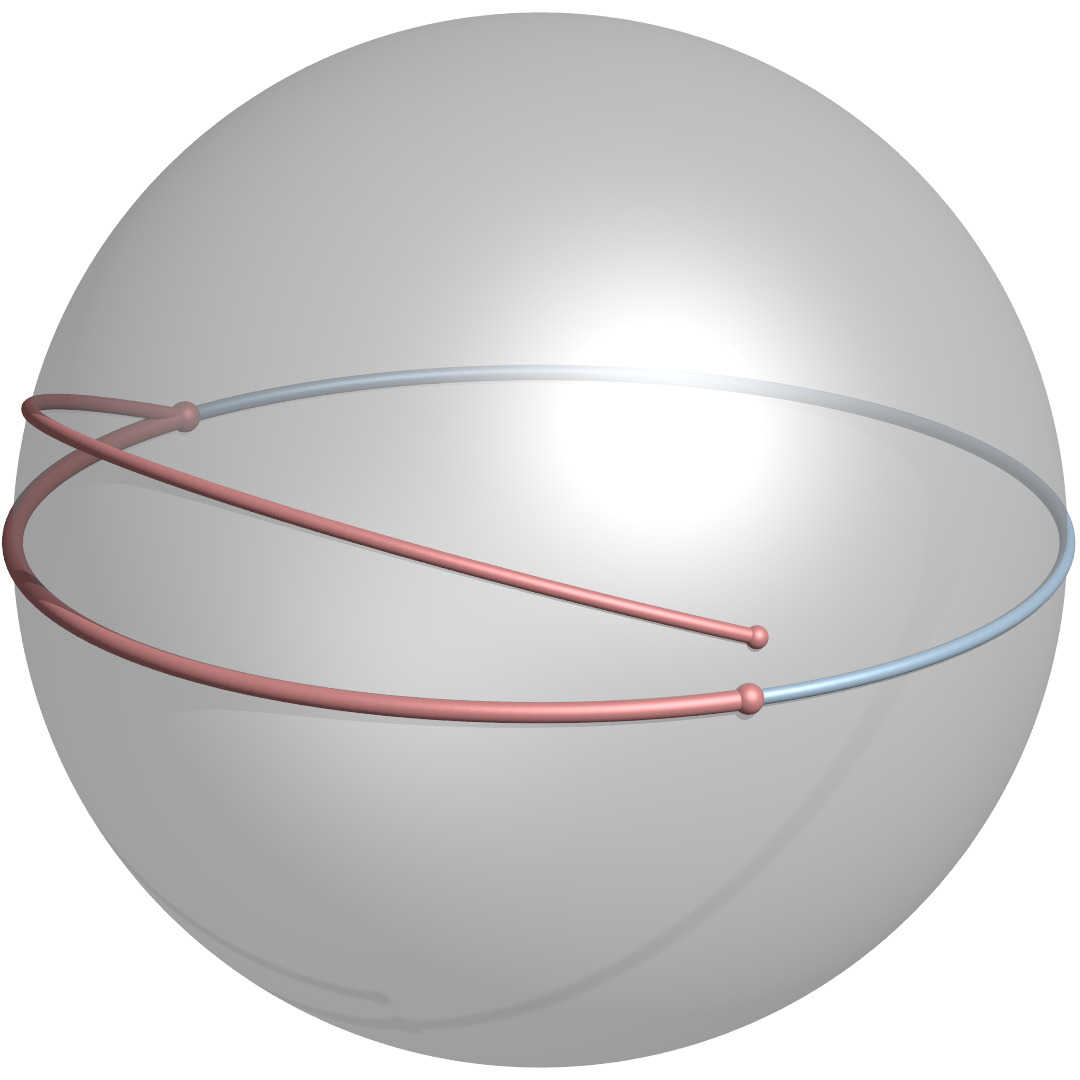
\includegraphics[width=4.00cm]{jacobi0.jpg}};
\node at (-1.3,0.7) {$x_0$};
\node at (0.8,-0.8) {$x_1$};
\node at (0,-2) [below] {a)\strut};
\end{scope}

\begin{scope}
\node at (0,0) {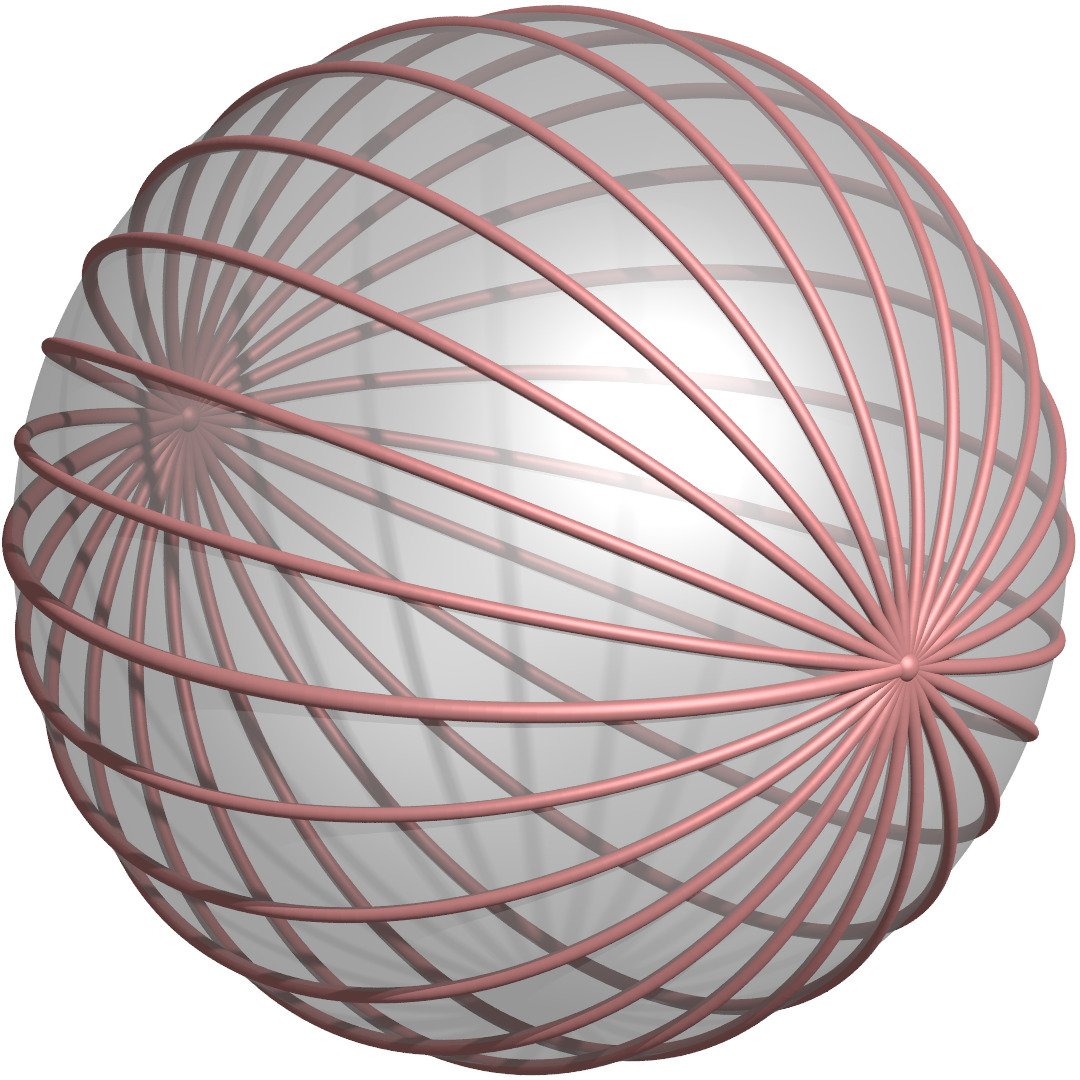
\includegraphics[width=4.00cm]{jacobi1.jpg}};
\node at (-1.2,0.2) {$x_0$};
\node at (1.4,-0.8) {$x_1$};
\node at (0,-2) [below] {b)\strut};
\end{scope}

\begin{scope}[xshift=4.2cm]
\node at (0,0) {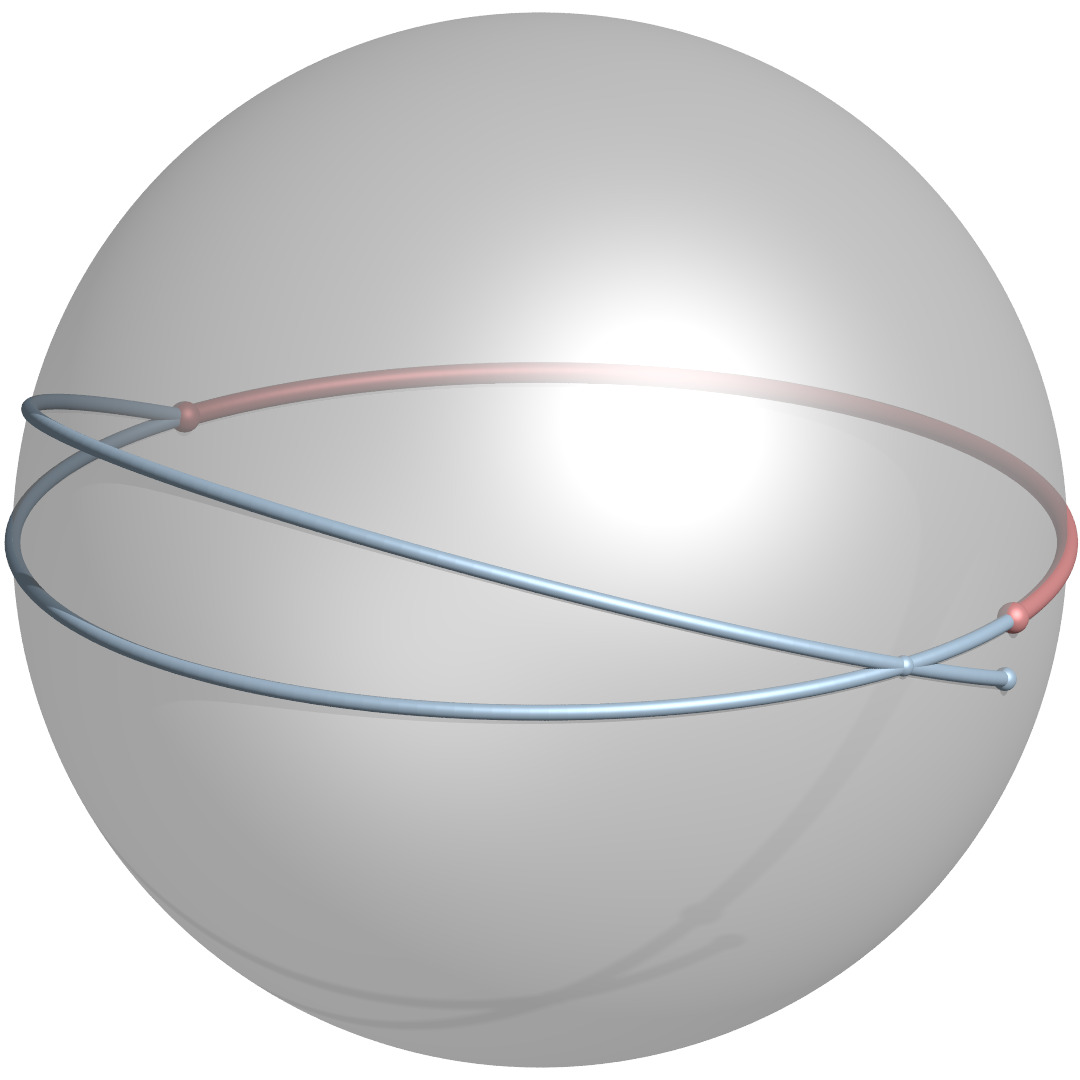
\includegraphics[width=4.00cm]{jacobi2.jpg}};
\node at (-1.3,0.7) {$x_0$};
\node at (1.3,-0.3) {$x_*$};
\node at (1.95,-0.5) {$x_1$};
\node at (0,-2) [below] {c)\strut};
\end{scope}

% Gitter
\ifthenelse{\boolean{showgrid}}{
\draw[step=0.1,line width=0.1pt] (-\breite,-\hoehe) grid (\breite, \hoehe);
\draw[step=0.5,line width=0.4pt] (-\breite,-\hoehe) grid (\breite, \hoehe);
\draw                            (-\breite,-\hoehe) grid (\breite, \hoehe);
\fill (0,0) circle[radius=0.05];
}{}

\end{tikzpicture}

\end{document}


Das durch Nullstellen einer Lösung $u_0(x)$ im Inneren des Intervalls
verursachte Phänomen kann sehr schön am Beispiel der kürzesten
Verbindung auf einer Kugeloberfläche illustriert werden.
Die kürzesten Verbindung zweier Punkte ist dort immer ein Grosskreisbogen.
Liegen die Punkte auf dem Äquator, dann liegt in Normalfall auch die
kürzeste Verbindung auf dem Äquator.

Seien jetzt $x_1$ und $x_2$ die geographische Länge von zwei Punkten
auf dem Äquator, zwischen denen die kürzeste Verbindung gesucht wird.
In Abbildung~\ref{buch:variation2:fig:jacobi} sind die möglichen
Situationen illustriert.
In a) ist das Intervall $|x_2-x_1|<\pi$, in diesem Fall ist die
das Intervall $[x_1,x_2]$ die kürzeste Verbindung und die 
Jacobi-Differentialgleichung hat keine Nullstellen im Inneren 
dieses Intervalls.

In c) ist das Intervall $|x_2-x_1|>\pi$, in diesem Fall ist das Intervall
$[x_1,x_2]$ die längste Verbindung.
Die Lösung $u_0(x)$ Jacbi-Differentialgleichung hat eine Nullstelle
bei $x_*=x_1+\pi$.
Mit dem Bogen in der oberen Halbkugel zwischen $x_1$ und $x_*$
gefolgt vom Äquatorabschnitt von $x_*$ bis $x_2$ kann man eine
alternative Verbindung herstellen, die zwar die gleiche Länge hat,
die aber durch Abrundung der Ecke bei $x_*$ verkürzt werden kann.
Dies ist die Erkenntnis aus der weierstrass-erdmannschen
Eckenbedingung für $u_1(x)$.
Die kürzeste Verbindung ist der komplementäre, rot eingezeichnete
Teil des Äquators.

In b) ist $x_2=x_1+\pi$.
In diesem Fall ist $u_0(x)$ eine Lösung, die die Randbedingung
$u_0(x_1)=u_0(x_2)=0$ erfüllt, sie kann also als Variation
für das ursprüngliche Integral verwendet werden.
Die variierten Lösungen sind alle rot eingezeichnet und haben,
da $u_0(x)$ die Jacobi-Differentialgleichung erfüllt, die gleiche
Länge.

Die Punkte $x_1$ und $x_*$ heissen {\em konjugierte} Punkte.
\index{konjugierter Punkt}%
Man kann das Phänomen auch so beschreiben: erweitert man den
Definitionsbereich über einen konjugierten Punkt hinweg, wird die
Lösung $y(x)$ ``instabil'', man kann den Wert des Funktionals
durch kleine Änderungen weiter senken.
Die Funktion $y(x)$ ist dann zwar immer noch ein kritischer Punkt,
des Funktionals, aber kein Minimum mehr.

%
% Lösungen ohne Nullstellen im Inneren
%
\subsection{Lösungen ohne Nullstellen im Inneren
\label{buch:variation2:jacobi:subsection:ohne}}
Wir nehmen jetzt an, dass $y(x)$ die starke Legendre-Bedingung
erfüllt und die Lösung $u_0(x)$ der zugehörigen
Jacobi-Differentialgleichung mit Anfangsbedingungen $u_0(x_1)=0$
und $u_0'(x_1)=1$ keine Nullstellen im Inneren des Intervalls
$[x_1,x_2]$ hat.
Wir wollen zeigen, dass unter diesen Voraussetzungen die zweite
Variation nicht negativ sein kann.

Die zweite Variation ist das Integral
\begin{align*}
\delta^2 I(y)
&=
\int_{x_1}^{x_2}
S(x) \eta(x)^2 + R(x) \eta'(x)^2
\,dx.
\intertext{Da die starke Legendre-Bedingung gilt, ist $R(x)>0$ und
kann daher ausgeklammert werden:}
&=
\int_{x_1}^{x_2}
R(x)
\biggl(
\eta'(x)^2 + \frac{S(x)}{R(x)}\eta(x)^2
\biggr)
\,dx
\end{align*}
Wenn man zeigen kann, dass die Klammer im Integranden ein Quadrat
ist, dann folgt, dass das Integral $\ge 0$ sein muss.

Wir berechnen zu diesem Zweck das Integral
\begin{align}
J&=
\int_{x_1}^{x_2} 
R(x) 
\biggl(
\eta'(x)
-\frac{u_0'(x)}{u_0(x)} \eta(x)
\biggr)^2
\,dx,
\label{buch:variation2:jacobi:eqn:Jquadrat}
\intertext{welches ausmultipliziert zu}
&=
\int_{x_1}^{x_2} 
R(x) 
\biggl(
\eta'(x)^2
-
2\frac{u_0'(x)}{u_0(x)} \eta(x) \eta'(x)
+\frac{u_0'(x)^2}{u_0(x)^2} \eta(x)^2
\biggr)
\,dx
\notag
\intertext{wird.
Die Faktoren mit $\eta$ im mittleren Term können kompakter
als $2\eta(x)\eta'(x)=(\eta(x))'$ geschrieben werden:}
&=
\int_{x_1}^{x_2}
R(x)
\biggl(
\eta'(x)^2
-
\frac{u_0'(x)}{u_0(x)}(\eta(x)^2)'
+
\frac{u_0'(x)^2}{u_0(x)^2}
\eta(x)^2
\biggr)
\,dx.
\notag
\intertext{Dadurch wird es jetzt möglich im mittleren Term
partielle Integration durchzuführen, bei der
$(\eta(x)^2)'$ aufgeleitet und $R(x)u_0'(x)/u_0(x)$ abgeleitet wird.
Man erhält wegen der Randbedingung $\eta(x_1)=\eta(x_2)=0$}
&=
\int_{x_1}^{x_2}
R(x)\eta'(x)^2
+
\underbrace{
\biggl(
\biggl(R(x)\frac{u_0'(x)}{u_0(x)}\biggr)'
+
R(x)
\frac{u_0'(x)^2}{u_0(x)^2}
\biggr)
}_{\displaystyle =A}
\eta(x)^2
\,dx.
\notag
\end{align}
In der
mit $A$ bezeichneten Klammer im Integranden berechnen wir die Ableitung
des ersten Terms mit der Produktregel für die Faktoren
\[
\biggl(
R(x)\frac{u_0'(x)}{u_0(x)}
\biggr)'
=
\biggl(
R(x)u_0'(x)
\cdot
\frac{1}{u_0(x)}
\biggr)'
=
(R(x)u_0(x))'\frac{1}{u_0(x)}
+
R(x)u_0(x)\biggl(\frac{1}{u_0(x)}\biggr)'
\]
und erhalten für
\begin{align*}
A
&=
\frac{1}{u_0(x)}
\frac{d}{dx} R(x) \frac{d}{dx}u_0(x)
+
R(x)u_0'(x)
\frac{d}{dx}\frac{1}{u_0(x)}
+
R(x)\frac{u_0'(x)^2}{u_0(x)^2}
\intertext{Da $u_0(x)$ eine Lösung der Jacobi-Differentialgleichung ist,
ist nach \eqref{buch:variation2:jacobi:eqn:jacobisl2}
der erste Term $=S(x)$ und damit}
A
&=
S(x)
-
R(x)u_0'(x)\frac{u_0'(x)}{u_0(x)^2}
+
R(x)\frac{u_0'(x)^2}{u_0(x)^2}
=
S(x).
\end{align*}
Eingesetzt im Integral erhalten wir schliesslich
\[
J
=
\int_{x_1}^{x_2}
R(x)\eta'(x)^2 + S(x) \eta(x)^2
\,dx
=
\delta^2 I(y).
\]
Die zweite Variation kann also als das Integral $J$ geschrieben
werden.
Der Integrand von $J$ in der Form
\eqref{buch:variation2:jacobi:eqn:Jquadrat}
ist $\ge 0$, denn $R(x)>0$ wegen der starken Legendre-Bedingung 
und der zweite Faktor, die Klammer, ist ein Quadrat und daher
auch $\ge 0$.
Somit folgt $J\ge 0$.
Damit haben wir den folgenden Satz gezeigt.

\begin{satz}[Jacobi-Bedingung]
Erfüllt eine Extremale $y(x)$ des Funktionals $I(y)$ die starke
Legendre-Bedingung und hat die Lösung $u_0(x)$ der Jacobi-Differentialgleichung
mit Anfangswerten $u_0(x_1)=0$ und $u_0'(x_1)=1$ im Inneren des
Intervalls $[x_1,x_2]$ keine Nullstellen, dann ist
$\delta^2 I(y)\ge 0$.
\end{satz}




%
% Kürzeste Verbindung auf einem Rotationskörper
%
\subsection{Kürzeste Verbindung auf einem Rotationskörper}
Seit über 2000 Jahren ist der Menschheit bekannt, dass die Erde
ungefähr die Form einer Kugel hat.
Erathostenes gelang es als Erstem, den Umfang der Erde mit
einem Fehler von weniger als $2\%$ zu bestimmen.
Die Entfernungsmessung auf einer Kugeloberfläche ist deutlich
komplizierter als auf einer Ebene.
Bereits im Altertum wurde die sphärische Trigonometrie entwickelt,
mit der sich Winkel und Seitenlägen von beliebigen Dreiecken auf
einer Kugeloberfläche berechnen lassen.
Van Brummelen \cite{buch:heavenly} gibt eine sorgfältige Einführung
in die Geschichte und die Anwendungen der sphärischen Geometrie.

\begin{beispiel}
Die kürzesten Verbindungen zweier Punkte auf einer Kugel ist ein
Grosskreis.
Liegen die Punkte weniger als $180^\circ$ Grad auseinander, gibt es
nur eine kürzeste Verbindung, das Längenfunktional nimmt ein
absolutes Minimum an.

Sind die Punkte jedoch Antipodenpunkte, dann gibt es unendliche viele
Grosskreise durch beide Punkte.
Das Längenfunktional hat kein absolutes Minimum mehr, die Drehung eines
Grosskreises um die Achse durch die beiden Punkte ist eine Variation,
die das Funktional nicht ändert.
Die beiden Punkte sind konjugierte Punkte.
\end{beispiel}

%
% Rotationsflächen
%
\subsubsection{Rotationsflächen}
Eine Rotationsfläche wird am einfachsten in Zylinderkoordinaten
$(\varphi,r,z)$
beschrieben.
Die $z$-Achse ist die Achse der Rotationsfläche, die Funktion $r(z)$
beschreibt einen Merdian.
Der Winkel $\varphi$ ist die geographische Länge.

\begin{beispiel}
Ein Rotationsellipsoid mit Äquatorradius $R$ ist gegeben durch die Funktion
\[
r(z)
=
\sqrt{R^2-\frac{z^2}{b^2}}.
\]
Der Poldurchmesser ist $2b$.
\end{beispiel}

%
% Kurvenparametrisierung
%
\subsubsection{Kurvenparametetrisierung}
Ziel der späteren Untersuchung ist herauszufinden, ob eine Linie
mit konstantem $z$ eine Verbindung geringster Länge zwischen den
Winkeln $\varphi_0$ und $\varphi_1$ ist.
Die Variation einer solchen Kurve ist charakterisiert durch die
Abweichung in $z$-Richtung.
Man darf daher annehmen, dass die Kurve durch eine Funktion $z(\varphi)$
mit $z(\varphi_1)=z(\varphi_2)=0$ beschrieben wird.
Ein Punkt der Kurve ist daher die Koordinaten
$(\varphi, r(z(\varphi)), z(\varphi))$
gegeben.

%
% Kurvenlänge
%
\subsubsection{Kurvenlänge}
Die Länge einer mit $t$ parametrisierten Kurve in Zylinderkoordinaten
wird durch ein Integral der Form
\begin{align}
l
&=
\int_{t_1}^{t_2}
\sqrt{
r^2
\dot{\varphi}(t)^2
+
\dot{r}(t)^2 
+
\dot{z}(t)^2
}\,dt
\notag
\intertext{gegeben.
Mit $\varphi$ als Parameter für die Kurve vereinfacht sich das Integral
auf}
l(z)
&=
\int_{\varphi_1}^{\varphi_2}
\sqrt{
r(z(\varphi))^2
+
r'(z(\varphi))^2 z'(\varphi)^2
+
z'(\varphi)^2
}
\,d\varphi
\label{buch:variation2:jacobi:bsp:laenge:l}
\\
&=
\int_{\varphi_1}^{\varphi_2}
\sqrt{
r(z(\varphi))^2 + z'(\varphi)^2 \bigl(1+r'(z(\varphi))^2\bigr)
}
\,d\varphi.
\notag
\intertext{Die Lagrange-Funktion dieses Funktionals ist}
L(\varphi,z,z')
&=
\sqrt{r(z)^2 + z^{\prime 2}\bigl(1+r'(z)^2\bigr)}.
\label{buch:variation2:jacobi:bsp:laenge:L}
\end{align}
Man beachte, dass $L$ nicht von $\varphi$ abhängt, was die
Euler-Lagrange-Differentialgleichung vereinfacht.

Die Länge des Breitenkreises $z=0$ ist das Integral von
$L(\varphi,0,0)$, also $l=(\varphi_2-\varphi_1)r(0)$.
Da der zweite Term unter der Wurzel von $L$ immer positiv
ist, kann die Kurvenlänge nur kleiner werden, wenn dar Radius
$r(z)$ für $z>0$ deutlich kleiner ist.
Wenn $r(z)$ mit zunehmendem $z$ nur langsam abnimmt, kann der
zweite Term die Länge immer noch grösser machen.
Die interessante Frage, die im Folgenden untersucht werden soll,
ist daher, wie schnell $r(z)$ abnehmen muss, damit $z(\varphi)=0$
nicht das Minimum des
Funktionals~\eqref{buch:variation2:jacobi:bsp:laenge:l}
ist.

%
% Euler-Lagrange-Differentialgleichung
%
\subsubsection{Euler-Lagrange-Differentialgleichung}
Für die Euler-Lagrange-Differentialgleichungen werden die partiellen
Ableitungen der Lagrange-Funktion wie folgt benötigt:
\begin{align}
\frac{\partial L}{\partial z}
&=
\frac{
r'(z) + z^{\prime 2}r''(z)r'(z)
}{
\sqrt{r(z)^2 + z^{\prime 2}(1+r'(z)^2)}
}
\label{buch:variation2:jacobi:rot:el-links}
\\
\frac{\partial L}{\partial z'}
&=
\frac{
z'(1+r'(z)^2)
}{
\sqrt{r(z)^2 + z^{\prime 2}(1+r'(z)^2)}
}.
\end{align}
Die Ableitung nach $z'$ muss nochmals abgeleitet werden.
Die Notation wird etwas unübersichlich, wir schreiben zunächst
\begin{align*}
Z(\varphi)
&=
z'(\varphi)\,(1+r'(z(\varphi))^2)
\\
N(\varphi)
&=
r(z(\varphi))^2
+
z'(\varphi)^2 (1+r'(z(\varphi))^2).
\end{align*}
Die gesuchte Ableitung von $L$ kann damit als
\begin{equation}
\frac{d}{d\varphi}\frac{\partial L}{\partial z'}
(\varphi,z(\varphi),z'(\varphi))
=
\frac{d}{d\varphi}\frac{Z(\varphi)}{\sqrt{N(\varphi)}}
=
\frac{
Z'(\varphi)N(\varphi)
-
\frac12
Z(\varphi)N'(\varphi)
}{
N(\varphi)^{\frac32}
}
\label{buch:variation2:jacobi:eqn:el2}
\end{equation}
geschrieben werden.
Auch der Term~\eqref{buch:variation2:jacobi:rot:el-links}
kann mit Hilfe von $N(\varphi)$ etwas kompakter geschrieben werden:
\begin{align*}
\frac{\partial L}{\partial z}
(\varphi,z(\varphi),z'(\varphi))
&=
\frac{
r'(z(\varphi)) + z'(\varphi)^2\,r''(z(\varphi))\,r'(z(\varphi))
}{\sqrt{N(\varphi)}}
\\
&=
\frac{
\bigl(r'(z(\varphi)) + z'(\varphi)^2\,r''(z(\varphi))\,r'(z(\varphi))\bigr)
\,
N(\varphi)
}{
N(\varphi)^{\frac32}
}.
\end{align*}
Damit kann man jetzt die Euler-Lagrange-Differentialgleichung 
kompakter schreiben.
Nach Multiplikation mit $N(\varphi)^{\frac32}$ bleibt
\begin{equation}
\bigl(
r'(z(\varphi)) + z'(\varphi)^2\,r''(z(\varphi))\,r'(z(\varphi))
\bigr)
\,
N(\varphi)
-
Z'(\varphi)N(\varphi) + \frac12 Z(\varphi)N'(\varphi)=0
\label{buch:variation2:jacobi:el-ZN}
\end{equation}
als Euler-Lagrange-Differentialgleichung.

Die Ableitungen von $Z(\varphi)$ und $N(\varphi)$ sind
\begin{align*}
Z'(\varphi)
&=
z''(\varphi)\,(1+r'(z(\varphi))^2)
+
2
z'(\varphi)^2\,r''(z(\varphi))\,r'(z(\varphi))
\\
N'(\varphi)
&=
2 r'(z(\varphi))\, r(z(\varphi))\, z'(\varphi)
+
2 z''(\varphi)\,z'(\varphi)\,(1+r'(z(\varphi))^2)
\\
&\qquad
+
2 z'(\varphi)^3\, r''(z(\varphi))\, r'(z(\varphi)),
\end{align*}
und müssen in \eqref{buch:variation2:jacobi:el-ZN} eingesetzt
werden. 

Die Berechnung von \eqref{buch:variation2:jacobi:el-ZN} wird
übersichtlicher, wenn die geschachtelten Funktionen nicht
mehr alle ausgeschrieben werden müssen.
Wir kürzen daher wieder $r'(z(\varphi)) = r'$ und $z'(\varphi)=z'$
und analog für höhere Ableitungen.
Dann werden die Terme für $Z(\varphi)$ und $N(\varphi)$
\begin{align*}
Z(\varphi)
&=
z'\,(1+r^{\prime 2}),
&&&
Z'(\varphi)
&=
z''\,(1+r^{\prime 2}) + 2z^{\prime 2}\,r''\,r',
\\
N(\varphi)
&=
r^2 + z^{\prime 2}(1+r^{\prime 2})
&&\text{und}&
N'(\varphi)
&=
2r'\,r\,z' + 2 z''\,z'\,(1+r^{\prime 2})+2 z^{\prime 3} r''\,r'.
\end{align*}

Wir sind nur daran interessiert zu prüfen, ob die
Euler-Lagrange-Differentialgleichung für die Funktion $z(\varphi)=0$
erfüllt ist.
Daher können wir $z(\varphi)=z=0$ und $z(\varphi)=z'=0$ setzen, dadurch
vereinfachen sich die Ausdrücke zu
\begin{align*}
Z(\varphi) &= 0
&
Z'(\varphi)
&=0
\\
N(\varphi) &= r(0)^2
&
N'(\varphi) &= 0.
\end{align*}
Damit wird die Euler-Lagrange-Differentialgleichung
\eqref{buch:variation2:jacobi:el-ZN}
\begin{equation}
r'(0)^2 r(0)^2 = 0.
\end{equation}
Die Funktion $z(\varphi)=0$ ist also nur dann eine Lösung der
Euler-Lagrange-Differential\-glei\-chung, wenn $r'(0)=0$ ist.

%
% Legendre-Bedingungen
%
\subsubsection{Legendre-Bedingungen}
Die Legendre-Bedingung fragt nach der zweiten Ableitung von $L$ nach $z'$.
Mit der Quotientenregel ist sie
\begin{align*}
\frac{\partial^2L}{\partial z^{\prime 2}}
&=
\frac{
(1+r'(z)^2)
\cdot
\sqrt{r(z)^2+z^{\prime 2}(1+r'(z)^2)}
-
z'(1+r'(z)^2)
\cdot
\displaystyle
\frac{
z'(1+r'(z)^2)
}{
\sqrt{r(z)^2 + z^{\prime 2}(1+r'(z)^2)}
}
}{
r(z)^2 + z^{\prime 2}(1+r'(z)^2)
}.
\intertext{Bringen wir die Quadratwurzel im zweiten Term in den
Nenner, indem wir den ersten Term damit erweitern, erhalten wir}
&=
\frac{
(1+r'(z)^2)
(r(z)^2+z^{\prime 2}(1+r'(z)^2))
-
z^{\prime 2}(1+r'(z)^2)^2
}{
\bigl(
r(z)^2 + z^{\prime 2}(1+r'(z)^2)
\bigr)^{\frac32}
}
\\
&=
\frac{
r(z)^2 ( 1 + r'(z)^2)
}{
\bigl(
r(z)^2 + z^{\prime 2}(1+r'(z)^2)
\bigr)^{\frac32}
}
>0.
\end{align*}
Die starke Legendre-Bedingung ist also immer erfüllt.

%
% Die Jacobi-Differentialgleichung
%
\subsubsection{Die Jacobi-Differentialgleichung}
Um die Jacobi-Differentialgleichung aufzustellen, müssen die Koeffizienten
$S(\varphi)$ und $R(\varphi)$ für die Funktion $z(\varphi)=0$ berechnet
werden.
Für $R(\varphi)$ benötigen wir die zweite Ableitung von $L$ nach $z'$,
die wir bereits berechnet haben, und finden
\begin{align*}
R(\varphi)
&=
\frac{
r(0)^2(1+r'(0)^2)
}{
r(0)^3
}
=
\frac{1+r'(0)^2}{r(0)}.
\end{align*}
$R(\varphi)$ ist also konstant.

Die Berechnung $P(\varphi)$ und $Q(\varphi)$ verlangt nach den anderen
zweiten Ableitungen von $L$, die aber auch wieder nicht von $\varphi$
abhängen werden.
Da auch $z(\varphi)$ und $z'(\varphi)$ für den untersuchten Breitenkreis
nicht von $\varphi$ abhängen, sind beide konstant.
Insbesondere wird die Ableitung $Q'(\varphi)=0$ sein, so dass
$S(\varphi)=P(\varphi)$ ist.
Es muss also nur noch $P(\varphi)$ bestimmt werden.

Die Ableitungen von $L$ sind
\begin{align*}
\frac{\partial L}{\partial z}
&=
\frac{
r'(z)(r''(z)z^{\prime 2}+r(z))
}{
\sqrt{(1+r'(z)^2)z^{\prime 2} +r(z)^2}
}
\intertext{mit der Quotientenregel}
\frac{\partial^2 L}{\partial z^2}
&=
\frac{
r''(z) (r''(z) z^{\prime 2} + r(z))
+
r'(z)(r'''(z) z^{\prime 2} + r'(z))
}{
\sqrt{
r(z)^2 + (1+r'(z)^2) z^{\prime 2}
}
}
-
\frac{
(r'''(z) z^{\prime 2} + r(z))^2
r'(z)^2
}{
(
r(z)^2
+
(1+r'(z)^2) z^{\prime 2}
)^{\frac32}
}.
\intertext{Wir brauchen diesen Ausdruck nur für $z=0$ und $z'=0$,
damit vereinfacht er sich zu}
P(\varphi)
&=
\frac{
r''(0)r(0)+r'(0)^2
}{
r(0)
}
-
\frac{
r(0)^2
r'(0)^2
}{
r(0)^3
}
=
r''(0).
\end{align*}
Die Jacobi-Differentialgleichung bekommt somit die Form
\begin{align}
\frac{d}{d\varphi}
R(\varphi)
\frac{d}{d\varphi}
u(\varphi)
&=
S(\varphi)
u(\varphi)
&&\Rightarrow&
u''(\varphi)
&=
\frac{S(\varphi)}{R(\varphi)} u(\varphi)
\notag
\\
&&&\Rightarrow&
u''(\varphi)
&=
\frac{r(0)r''(0)}{1+r'(0)^2}
u(\varphi).
\label{buch:variation2:jacobi:rot:lambda}
\end{align}
Der Bruch auf der rechten Seite bestimmt die Lösungen vollständig.
Falls $r''(0) > 0$ ist, ist die konvex und damit kann sie keine
weitere Nullstellen haben.

%
% Die Lösungen der Jacobi-Differentialgleichung
%
\subsubsection{Die Lösungen der Jacobi-Differentialgleichung und die konjugierten Punkte}
Die Differentialgleichung
\[
u''(x) = -\lambda u(x)\qquad\text{mit $u(\varphi_1)=0$}
\]
hat die Lösung 
\[
u(\varphi)
=
A\sin \sqrt{\lambda}(\varphi-\varphi_1),
\]
mit Nullstellen bei $\varphi_1 + \pi k/\sqrt{\lambda}$ mit $k\in\mathbb{Z}$.
Daraus können wir jetzt ablesen, dass die konjugierten Punkte bei
$\varphi_1\pm \pi/\sqrt{\lambda}$ zu finden sind.
Mit dem Wert von $\lambda$ aus~\eqref{buch:variation2:jacobi:rot:lambda}
erhalten wir 
\begin{equation}
\Delta\varphi
=
\pi
\sqrt{-\frac{1+r'(0)^2}{r(0)r''(0)}}
\label{buch:variation2:jacobi:rot:abstand}
\end{equation}
für den Winkelabstand zwischen konjugierten Punkten.

%
% Konjugierte Punkte auf der Einheitskugel
%
\subsubsection{Konjugierte Punkte auf der Einheitskugel}
Die Einheitskugel ist der Fall
\begin{equation}
\left.
\begin{aligned}
r(z)
&=
\sqrt{1-z^2}
&&\Rightarrow&
r(0)&=1
\\
r'(z)
&=
-
\frac{z}{\sqrt{1-z^2}}
&&\Rightarrow&
r'(0)&=0
\\
r''(z)
&=
-
\frac{1}{(1-z^2)^{\frac32}}
&&\Rightarrow&
r''(0)&=-1
\end{aligned}
\quad
\right\}
\qquad\Rightarrow\qquad
\Delta
=
\pi,
\end{equation}
die konjugierten Punkte sind also wie erwartet Antipodenpunkte.

%
% Konjugierte Punkte auf einem Rotationsellipsoid
%
\subsubsection{Konjugierte Punkte auf einem Rotationsellipsoid}
Ein Rotationsellipsoid mit Äquatorradius $1$ und Polradius $b$
entsteht für die Funktion $r(z)=\sqrt{1-z^2/b^2}$.
Die Berechnung des Winkelabstands für die konjugierten Punkte
ergibt
\begin{equation}
\left.
\begin{aligned}
r(z) &= \sqrt{1-\frac{z^2}{b^2}}
&&\Rightarrow&
r(0) &= 1
\\
r'(z) &= -\frac{z}{\displaystyle b^2\sqrt{1-\frac{z^2}{b^2}}}
&&\Rightarrow&
r'(0) &= 0
\\
r''(z)
&=
-\frac{1}{b^2\biggl(\displaystyle1-\frac{z^2}{b^2}\biggr)^{\frac32}}
&&\Rightarrow&
r''(0) &= -\frac{1}{b^2}
\end{aligned}
\quad
\right\}
\qquad\Rightarrow\qquad
\Delta
=
\pi b.
\end{equation}
Wenn das Ellipsoid also einen kleineren Polradius als $1$ hat, dann
sind die konjugierten Punkt näher als einen halben Umfang vom
Ausgangspunkt entfernt.

Man kann dieses Resultat auch wie in
Abbildung~\ref{buch:variation2:fig:geodaeten} visualisieren.
%
% geodesics.tex
%
% (c) 2024 Prof Dr Andreas Müller
%
\begin{figure}
\centering
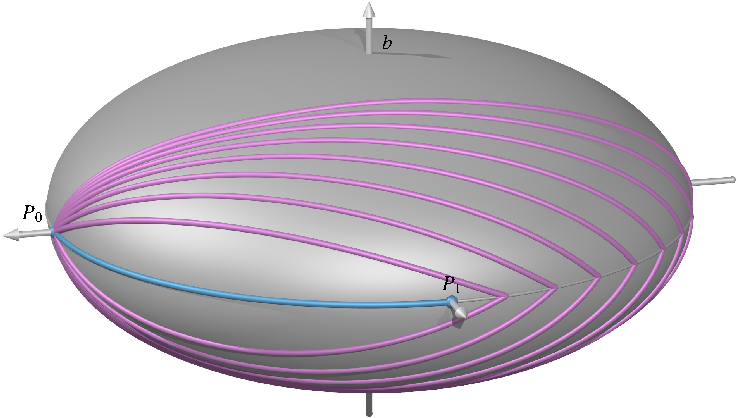
\includegraphics{chapters/060-variation2/examples/geodesics.pdf}
\caption{vom Punkt $P_0$ ausgehende Geodäten auf einem Rotationsellipsoid
mit Äquatorradius $1$ und Polradius $b$.
Die Kurve entlang des Äquators (blau) ist eine Lösung der
Euler-Lagrange-Differentialgleichung und sie erfüllt immer die starke
Legendre-Bedingung, aber das Jacobi-Kriterium ist nicht erfüllt, wenn 
sie länger als $b\pi$ wird.
Bei dieser Länge findet man den konjugierten Punkt $P_1$, ab
dieser Länge sind die rosaroten Geodäten kürzer.
\label{buch:variation2:fig:geodaeten}}
\end{figure}
%
Der Äquator ist eine Lösung der Euler-Lagrange-Differentialgleichung
für die Verbindungen zwischen den Punkten $\varphi_1$ und $\varphi_2$.
Sie wird für $b <= (\varphi_2-\varphi_1)/\pi$ instabil und es gibt
eine kürzere Verbindung, die nicht entlang dem Äquator verläuft.
In Abbildung~\ref{buch:variation2:fig:geodaeten} beginnen alle
Geodäten beim Punkt $P_0$.
Der Punkt $P_2$ ist der konjugierte Punkt, für Punkte $P$ jenseits dieses
Punktes gibt es eine kürzere Verbindung von $P_1$ zu $P$.


%
% Die Gestalt der Erde
%
\subsubsection{Die Gestalt der Erde}
Die Erde ist aber nicht eine Kugel, sondern eher ein Rotationsellipsoid,
der Durchmesser entlang der Achse ist verschieden vom Durchmesser des 
Äquators.
\index{Erde}%
Im 17. Jahrhundert gab es einen wissenschaftlichen Disput darüber,
ob der Durchmesser entlang der Achse kleiner oder grösser als der
Äquatordurchmesser ist.
Newton und Huygens hatten aufgrund der allgemeinen Mechanik eine Abplattung
der Erde vorhergesagt, die durch von Jean Richter und Philipp de La Hire
\index{Richter, Jean}%
\index{de La Hire, Philipp}%
durch die erste Vermessung des Merdianbogens durch Paris bestätigt 
worden war.
Die Sache war aber immer noch nicht vollständig geklärt.
Der Astronom Jacques Cassini schloss zu Beginn des 18. Jahrhunderts,
\index{Cassini, Jacques}%
dass der Polradius grösser als der Äquatorradius sein müsse.
König Ludwig XV.~beauftragte daher Maupertuis mit einer Expedition
\index{Louis XV.}%
\index{Maupertuis}%
nach Lappland.
\index{Lapland}%
Als Teil der Expedition soll der Abstand zweier Breitengrade
vermessen werden.
Wenn der Radius im hohen Norden immer schneller abnimmt, wird auch die Länge
eines Merdianbogens zu vorgegebenem Winkel kürzer.
Die Expedition von Maupertuis und eine zeitgleich stattfindende Expedtion
nach Ecuador bestätigten beide die Abplattung.
\index{Ecquador}%




